%% TITOLO
\section{Sistemi Autonomi}
\label{sec:Sistemi Autonomi}

\subsection{Order From Noise (Homage to Heinz Von Foerster)}
\label{sec:Order From Noise (Homage to Heinz Von Foerster)}

Nel capitolo precedente, attraverso la composizione e gli studi di Agostino Di Scipio, 
abbiamo potuto osservare che cosa si intende, e come viene organizzato, 
un sistema con non linearità provenienti dal mondo fisico; aperto al suo ambiente esterno 
che diviene in questo caso lo spazio stesso della performance.
Sempre in riferimento alla cibernetica di secondo ordine,
abbiamo già parlato del fatto che nessun sistema è separabile e 
isolabile da un suo ambiente circostante, 
ma abbiamo osservato anche come il concetto di spazio di un sistema sia 
qualcosa di molto complesso, poiché il concetto stesso di complessità
sta a significare in un sistema che questo sia composto da una rete d'interazioni dinamiche, 
ma che il comportamento dell'insieme potrebbe non essere prevedibile in base al comportamento 
dei diversi componenti tipicamente in relazione fra loro.

Mentre, nel caso di Agostino Di Scipio, lo spazio del sistema che ne contiene le sue relazioni 
è costituito principalmente dal mondo fisico, 
in questo capitolo osserveremo come, per lo spazio di un sistema, 
si possa intendere anche uno spazio latente, 
che traccia le sue relazioni tra le parti in uno spazio virtuale interamente programmato nel software. 
In questo caso, l'ambiente digitale che racchiude il sistema all'interno e le sue relazioni 
tra gli agenti è interamente costituito solo dal DSP, 
inclusi i metodi per la generazione delle relative non linearità.
Ho voluto approfondire questo metodo attraverso il lavoro compositivo e gli studi di Dario Sanfilippo, 
specialista di sistemi di \emph{feedback}, esecutore e compositore. 
I suoi lavori riguardano principi di autopoiesi, evolvibilità e costruttivismo radicale nella progettazione 
di reti di \emph{feedback} audio complesse. 

La modalità con cui andrò a discutere in questo capitolo la composizione di questi
sistemi autonomi, appartenenti anche questi alla più vasta categoria dei CASes (Complex Adaptive Systems), 
è ponendo un focus su un particolare lavoro di Dario Sanfilippo, Order From Noise \textit{(Homage to Heinz Von Foerster)}.

Order From Noise è un progetto che implementa uno 
dei primi prototipi di Dario Sanfilippo basati sull'idea dell'\textit{adattattività dinamica}. 
Questo lavoro del compositore si basa sull'idea che i sistemi adattivi complessi, 
che sono emergenti per definizione, siano essenziali per raggiungere innovazioni formali, 
performative e tecniche, nel contesto della performance in live electronics e nella composizione musicale in generale. 
\footcite{sanfilippo_time-variant_2018}
I CASes si dicono adattivi quando sono composti da una rete dinamica 
di interazioni dove i singoli agenti sono interconnessi fra loro, interagendo individualmente
o collettivamente, possono cambiare il loro stato in risposta a variazioni nell'ambiente o
degli altri agenti connessi. 
Questo tipo di relazioni nel sistema è comune sia nell'opera di Agostino Di Scipio,
in cui abbiamo visto precedentemente come lo stato dei singoli agenti nel sistema 
cambi al variare delle condizioni nell'ambiente circostante portando a
cambiamenti di stato globali del sistema, che nel lavoro di Dario Sanfilippo.
Altro importante aspetto in comune qui con l'opera di Agostino Di Scipio,
è il tipo di rapporto che ha l'uomo con la macchina, che viene respinto nella visione in cui è il primo
ad essere totalmente a controllo del secondo, per essere sostituito da un concetto 
d'interazione Uomo-Macchina-Ambiente, chiamato da Dario Sanfilippo Ibridazione: 
una condizione in cui umano e macchina cooperano per far emergere la performance. 
Nel caso delle opere di Dario Sanfilippo, tuttavia, l'estetica dei suoi lavori è interamente subordinata
al disegno del sistema stesso, che di volta in volta, emerge da fenomeni musicali che sono il risultato
del tipo d'interazione che viene a crearsi fra il performer e il disegno del sistema che si era reso necessario
in partenza. 

In alcuni casi, questa idea viene portata alle sue estreme conseguenze con opere in cui la macchina è l'unica 
ente che esegue, come accade per il brano presentato qui.

\begin{quote}
    Order from noise (2017) is based on a time-variant feedback delay network containing a 
    set of entangled nonlinear processing algorithms for audio and information signals. 
    The work is an example of autonomous self-performing system and it is realised by
    feeding the network with one millisecond of background noise from the performance
    environment. The initial recirculating noise impulse is what entirely determines the
    formal evolutions of the system which have substantially different long-term developments 
    for each different noise impulse. An approach to present the work live is that
    of reinitialising the system a number of times for a period of about three-five minutes
    to show its sensitivity to initial conditions and the long-term divergence between the
    formal structures.\footcite{sanfilippo_time-variant_2018}
\end{quote}

Rispetto al sistema discusso nel capitolo precedente, 
come già accennato c'è una sostanziale differenza nel concetto di spazio
o ambiente del sistema. 
Come appena detto, Order From Noise è basato su una \textit{feedback delay network} 
tempo-variante, vale a dire che ci ritroviamo di fronte ad un un sistema il cui
funzionamento stesso cambia nel tempo, a differenza dei sistemi tempo-invarianti
dove seppur l'output del sistema può cambiare nel tempo, 
il loro funzionamento e l'ambiente che contiene il sistema rimane inalterato.
In parole semplici: lo spazio del sistema in Order From Noise può variare nel tempo
rendendo imprevedibile il suo funzionamento a partire da una determinata condizione 
iniziale.
Per questo motivo il performer non avrà un grande margine di prevedibilità 
nel comportamento del sistema a differenza dei sistemi tempo-varianti,
ma saprà che per le stesse condizioni iniziali, il sistema qui totalmente
deterministico, riporterà sempre le stesse evoluzioni formali.
Proprio come nei sistemi caotici emersi dalla teoria del caos introdotti all'inizio di questa tesi,
che seppur governati da leggi deterministiche, 
sono in grado di esibire un'empirica casualità nell'evoluzione delle variabili dinamiche. 

\subsection{Audio Information Processing}
\label{sec:Audio Information Processing}
Come già accennato nello scorso capitolo, l'\textit{Audio Information Processing};
ovvero la capacità di un sistema di elaborare le informazioni
tremite la \textit{feature extraction}, è un dato fondamentale nella creazione 
di un CAS, che ne determina le sue capacità congitive e di auto-osservazione
rispetto all'ambiente. 
L'uso creativo dei CASes in Musica,
e la loro stretta connessione con l'informazione,
ha favorito lo sviluppo di techniche algoritmiche per l'\textit{Audio Information Processing} 
e l'analisi di comportamenti, sia ad alto e basso livello.

\begin{quote}
    The low-level algorithms provide a continuous measure of the features and can operate
    with short analysis frames. The high-level algorithms, on the other hand, are original designs informed both perceptually
    and by complexity theory for the analysis of musically meaningful information, both in short sounds or articulated
    streams with long-term nontrivial variations.\footcite{sanfilippo_time-domain_2021}
\end{quote}

Alcuni primi esempi storici,
sono ad esempio le performance in live electronics di Gordon Mumma, 
come: Diastasis, as in Beer (1966), e Hornpipe (1967), 
dove vengono implementate techniche di amplitude following utilizzate 
poi per pilotare parametri nelle unità di generazione del suono.\footcite{sanfilippo_time-domain_2021}
Arrivando fino ai sistemi di Agostino Di Scipio, che nello studio del suo
\emph{feedback study} ci ha dato modo di approfondire e scoprire
tutti quei meccanismi e tutte quelle particolari funzioni che hanno la responsabilità
di generare segnali di controllo nei suoi sistemi. 

Dario Sanfilippo ha discusso in più articoli l'utilizzo dell'\textit{Information Processing} 
nei CASes, sia in senso generale\footcite{sanfilippo_time-domain_2021}, 
parlando di implementazioni più tipiche come: 
centroide spettrale, rumorosità, diffusione spettrale a basso livello, eterogeneità e
complessità per l'alto livello.
Che come in questo caso nell'utilizzo specifico di queste tecniche 
in un suo sistema:

\begin{quote}
    These signals, often based on
    their perceptual characteristics and their relationship with the domains of the variables
    in the processing units, are mapped to certain ranges and then used to control the state
    of the components in a large network. (See Di Scipio (2003) for a detailed discussion
    on this method). Using infrasonic signals to pilot these variables is highly desirable if
    not necessary, for high-rate, sudden changes in the DSP parameters would produce an
    output with a continuously large and homogeneous spectral band, so it would not be
    possible to perceive the state variations in the long-term.
    The information and audio processing algorithms implemented, the specific connections 
    between the control signals and the variables, the linear and nonlinear mapping strategies 
    used as well as the network topologies, all these elements determine the
    infrastructure of a system. In a large network, these elements can already provide a high
    number of configurations and an even larger number of possible states that a system
    can reach. That, theoretically, could be considered as something that guarantees a good
    variety and complexity in the long-term behaviour of a system, albeit the practical case
    tends to be much different from the ideal scenario.\footcite{sanfilippo_time-variant_2018}
\end{quote}

Nel suo articolo su Order From Noise, Sanfilippo discute tutte le unità utilizzate
nel suo sistema e il loro ruolo all'interno della rete.
Partendo dalla descrizione di queste nell'articolo, tratterò ora una parte più operativa 
implementando queste tecniche nel linguaggio di programmazione FAUST (Grame), 
con un particolare focus su tutte tutte quelle \textit{feature extraction}
che nell'implementazione della rete permettono al sistema 
(nonostante questo sia chiuso rispetto all'ambiente esterno) 
di mantenersi in uno stato emergente manifestando comportamenti nuovi,
e di stabilità rimanendo sempre in dei range controllati tramite \emph{feedback positivi} e \emph{negativi}.

\begin{figure}[h!]
\begin{center}
    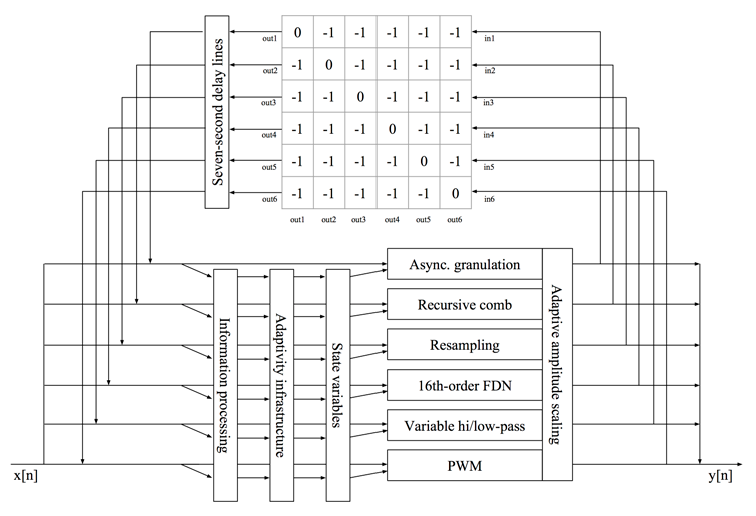
\includegraphics[width=14cm]{figures/OFNnetwork.pdf}
    \caption{Schema della rete di Order From Noise}
    \end{center}
\end{figure}

La rete di Order From Noise ha sei nodi, ognuno dei quali contiene due unità in cascata, 
contenenti i seguenti algoritmi di elaborazione audio: 
\textit{asynchronous granulation, recursive comb filtering, variable high-pass/low-pass filtering, pulse-width mod-
ulation (PWM), resampling and 16th-order feedback delay network (FDN) processing.} 

A parte le unità di elaborazione del suono,
in questo sistema, l'\textit{Information Processing} utilizzato per generare i 
segnali di controllo è diverso
dalle implementazioni tipiche riportate precedentemente nel corso di questa tesi;
piuttosto che calcolare \textit{feature extraction} come l'RMS, la diffusione spettale, ecc. 
Dario Sanfilippo utilizza in questo sistema una sorta di Low Frequency Oscillator
non lineare dipendente dal segnale in ingresso.
Questo comportamento viene ottenuto utilizzando un filtro Lowpass per far 
passare solo le componenti energetiche di un segnale sotto la soglia di 1Hz,
come ad esempio segnali a 0.01Hz, il segnale risultante viene poi processato
tramite normalizzazione dinamica per essere riportato ad una soglia in ampiezza
in un range fra [-1; 1],
viene elevato a una potenza relativamente grande per forzarlo intorno a 0,
ed infine utilizzato per pilotare la frequenza di un fasore.

\vspace{0.5cm} 
\lstinputlisting[breaklines, frame=trBL, caption={non linearità in Order From Noise}]
{codes/OFNnonLinearity.dsp}

La funzione \verb|lowFreqNoise(x)| accetta un segnale in ingresso
facendolo passare per uno stadio di 4 filtri Lowpass a cascata,
dove la stessa frequenza di taglio viene passata esternamente 
dalla variabile \verb|refPeriod|.
Il segnale passa poi per il normalizzatore dinamico composto dalle funzioni
\verb|noiseRMS(x)| e \verb|normRMS(x)|,
questo tipo di normalizzazione dinamica si basa sulla stima RMS e ha due ingressi,
uno è il segnale di riferimento, e l'altro è il segnale che deve essere normalizzato sulla base
del segnale di riferimento fornito, ovviamente,
la finestra RMS deve essere abbastanza grande a seconda della lentezza del
segnale che deve essere normalizzato.

Per comprendere meglio i meccanismi alla base
della normalizzazione dinamica,
andrò a discutere ora il caso più generico
di una normalizzazione di picco in DSP. 

Partendo dall'algoritmo basilare del \textit{Peakholder} in IIR discusso nel precedente capitolo. 
L'ampiezza del picco di un segnale può essere normalizzata secondo la seguente espressione 

\begin{align*}
    y_{1}(t) = (1/(\max\left( y_{1}(t\!-\!1), \left\lvert{x(t)}\right\rvert \right))) * x(t) 
\end{align*}

dove \textit{x} è il segnale in ingresso, e \textit{y} il segnale sia in uscita che reiterato nella funzione. 

Per prima cosa si calcola con il \textit{Peakholder} il picco massimo del segnale,
tracciandone il profilo di ampiezza campione per campione,
e a seguito si divide poi il risultato per 
un fattore per cui si desidera riscalare il segnale, in questo caso una costante 1.
Ed infine il profilo di ampiezza risultante da questa operazione verrà moltiplicato 
per lo stesso segnale in ingresso, incrementando o riducendo l'ampiezza di questo in base al risultato dell'operazione, 
e ridimensionando grazie a questo processo l'ampiezza di tutti i campioni del segnale, 
in modo tale che l'ampiezza del picco abbia un valore pari a [1, -1].

\vspace{0.5cm} 
\lstinputlisting[breaklines, frame=trBL, caption={Algoritmo di normalizzazione di picco tramite \textit{Peakholder} ad 1 campione di ritardo}]
{codes/PeakNormalizationIIR.dsp}

\begin{figure}[h!]
\begin{center}
    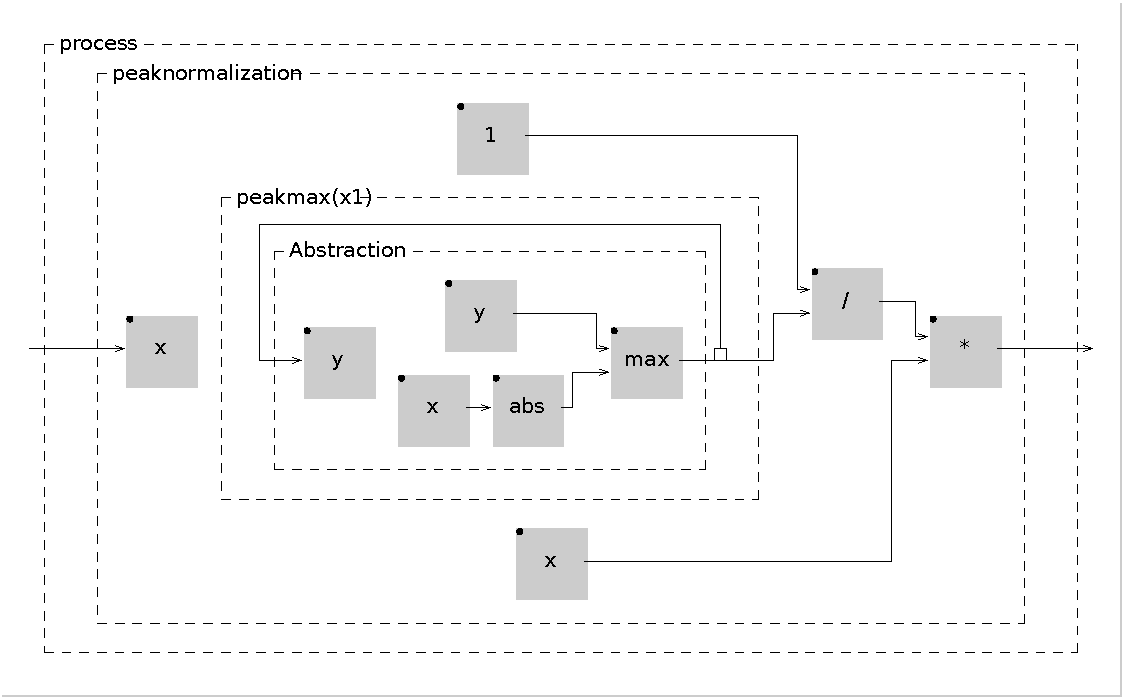
\includegraphics[width=14cm]{figures/PeakNormalizationIIR.pdf}
    \caption {Topologia del normalizzatore di picco tramite \textit{Peakholder} ad 1 campione di ritardo}
\end{center}
\vspace{0.5cm}
\end{figure}
    
Proprio come nell'algoritmo del \textit{Peakholder} ad 1 campione di ritardo, 
il problema di questa applicazione dipende dal fatto che nel segnale
complessivo possano permanere contributi spuri che alterino il risultato
della normalizzazione, e che si possa generare aliasing a causa di una mancata
funzione di smoothing del segnale.
Per questi motivi nelle unità della rete di Order From Noise 
che implementano al proprio interno meccanismi di \emph{feedback},
e per raggiungere quindi una stabilità globale della rete,
è presente un tipo di limiter dinamico chiamato da Dario Sanfilippo
col nome di \textit{Lookahead Limiter}, che a differenza dell'algoritmo
appena discusso ha un comportamento adattivo.
Questo tipo di Algoritmo viene descritto da Dario Sanfilippo sia nell'articolo 
di Musica/Tecnologia dell' 11-12 (2017-2018) che parla di Order From Noise 
citato precedentemente,\footcite{sanfilippo_time-variant_2018}
che nel suo blog, dove ne riporta un implementazione fatta nel linguaggio di programmazione
Pure Data.

\begin{quote}
    Recently, I have decided to try the design of a limiter based on a post by IOhannes Zmölnig who, 
    in turn, has based his design on the thesis project by Peter Falkner: 
    Entwicklung eines digitalen Stereo-Limiters mit Hilfe des Signalprozessors DSP56001.
    This design is based on a peak-hold module with an exponential decay curve...
    The first step in a lookahead limiter is to delay the input signal so 
    that the attenuating curve can anticipate fast peaks. 
    The amplitude profile of the input signal is obtained by combining a peak-hold module 
    – something that holds a peak for a certain time until a new peak is detected – 
    with a peak envelope one to have a smooth decay when signals transition to lower peaks. 
    Here, after, the peak-hold module, 
    I am also using a one-pole low-pass filter with a period matching that of the input delay 
    so that peaks and input signal are synchronised and the attack is slightly smoothed out... 
    The peak envelope can easily be implemented as a single feedback loop through which the detected peaks recirculate \\
    (Lookahead limiting in Pure Data - July 2, 2017
    \footcite{https://www.dariosanfilippo.com/blog/2017/lookahead-limiting-in-pure-data/})
\end{quote}

Per implementare il \textit{Lookahead Limiter} 
sono dunque richieste due unità distinte
combinate fra loro in feedforward con un filtro onepole Lowpass fra le due,
un \textit{Peakholder} con una finestra che mantiene il picco massimo del segnale e
che viene resettata da un timer, 
e un \textit{Peakenvelope} che ha invece un decadimento 
basato su \textit{tau} all'interno della retroazione; sono entrambe due
unità ottimizzate del nostro algoritmo \textit{Peakholder} ad 1 campione di ritardo,
e che combinate fra loro consentono di rilevare sia i transienti di attacco rapidi, 
che al contempo di avere una lunga fase di decadimento per i suoni sostenuti e lenti.

Il \textit{Peakenvelope} può essere ottenuto modificando 
la retroazione dell'algoritmo \textit{Peakholder}, moltiplicandola per 
un fattore di decadimento come nella seguente formula 

\begin{align*}
    y_{1}(t) = \max\left( k_{1} * y_{1}(t\!-\!1), \left\lvert{x(t)}\right\rvert \right)
\end{align*}
dove 
\begin{align*}
    k_{1} = {0.001}^{\frac{ST}{T}} 
\end{align*} 

è la formula del decadimento RT60, 
e dove \textit{T} rappresenta il tempo di decadimento desiderato in secondi, 
mentre \textit{ST} rappresenta la durata di un campione in secondi per la frequenza di campionamento corrente.
Come nelle altre formule del \textit{Peakholder}, \textit{x} è il segnale in ingresso, 
e \textit{y} il segnale sia in uscita che reiterato nella funzione stessa. 

A seguito l'algoritmo in Faust del \textit{Peakenvelope}.

\vspace{0.5cm} 
\lstinputlisting[breaklines, frame=trBL, caption={Algoritmo di \textit{Peakenvelope} con Decay RT60}]
{codes/PeakEnvelope.dsp}

\begin{figure}[h!]
\begin{center}
    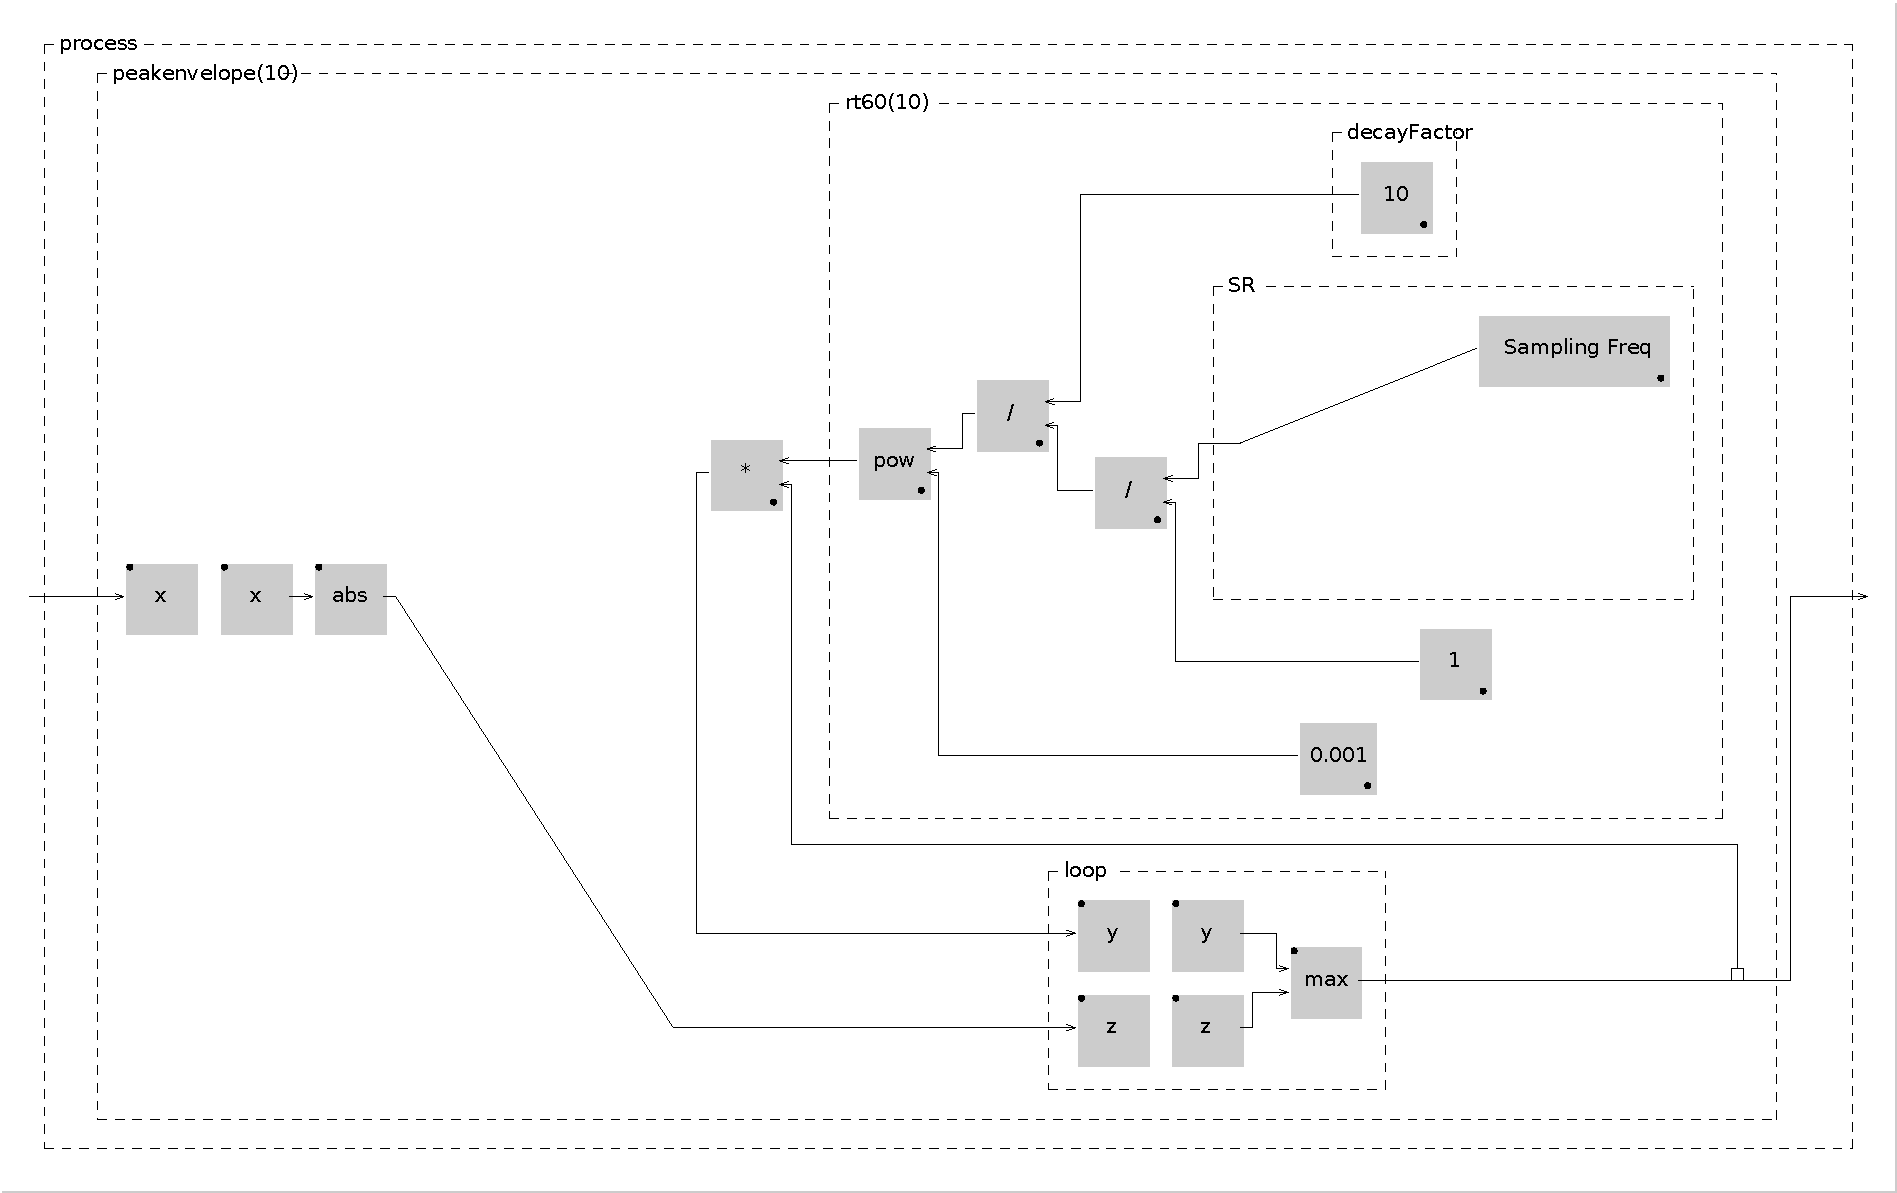
\includegraphics[width=15cm]{figures/PeakEnvelope.pdf}
    \caption{Topologia del \textit{Peakenvelope} con Decay RT60}
\end{center}
\vspace{0.5cm}
\end{figure}

per quanto riguarda invece l'algoritmo del \textit{Peakholder} adattivo, è un po' meno semplice. 
Il \textit{Peakholder} verificherà se l'ingresso è maggiore o uguale all'uscita e, 
se la condizione è vera, aggiornerà il picco e ripristinerà un timer. 
Quando la condizione invece è falsa, 
inizierà il suo countdown e, allo scadere del tempo, se non è stato rilevato alcun nuovo picco, 
qualsiasi valore nell'ingresso corrente verrà impostato come nuovo picco.

\lstinputlisting[breaklines, frame=trBL, caption={Algoritmo del \textit{Peakholder} (adattivo) con Timer}]
{codes/PeakHolderAdaptive.dsp}

\begin{figure}[h!]
    \begin{center}
        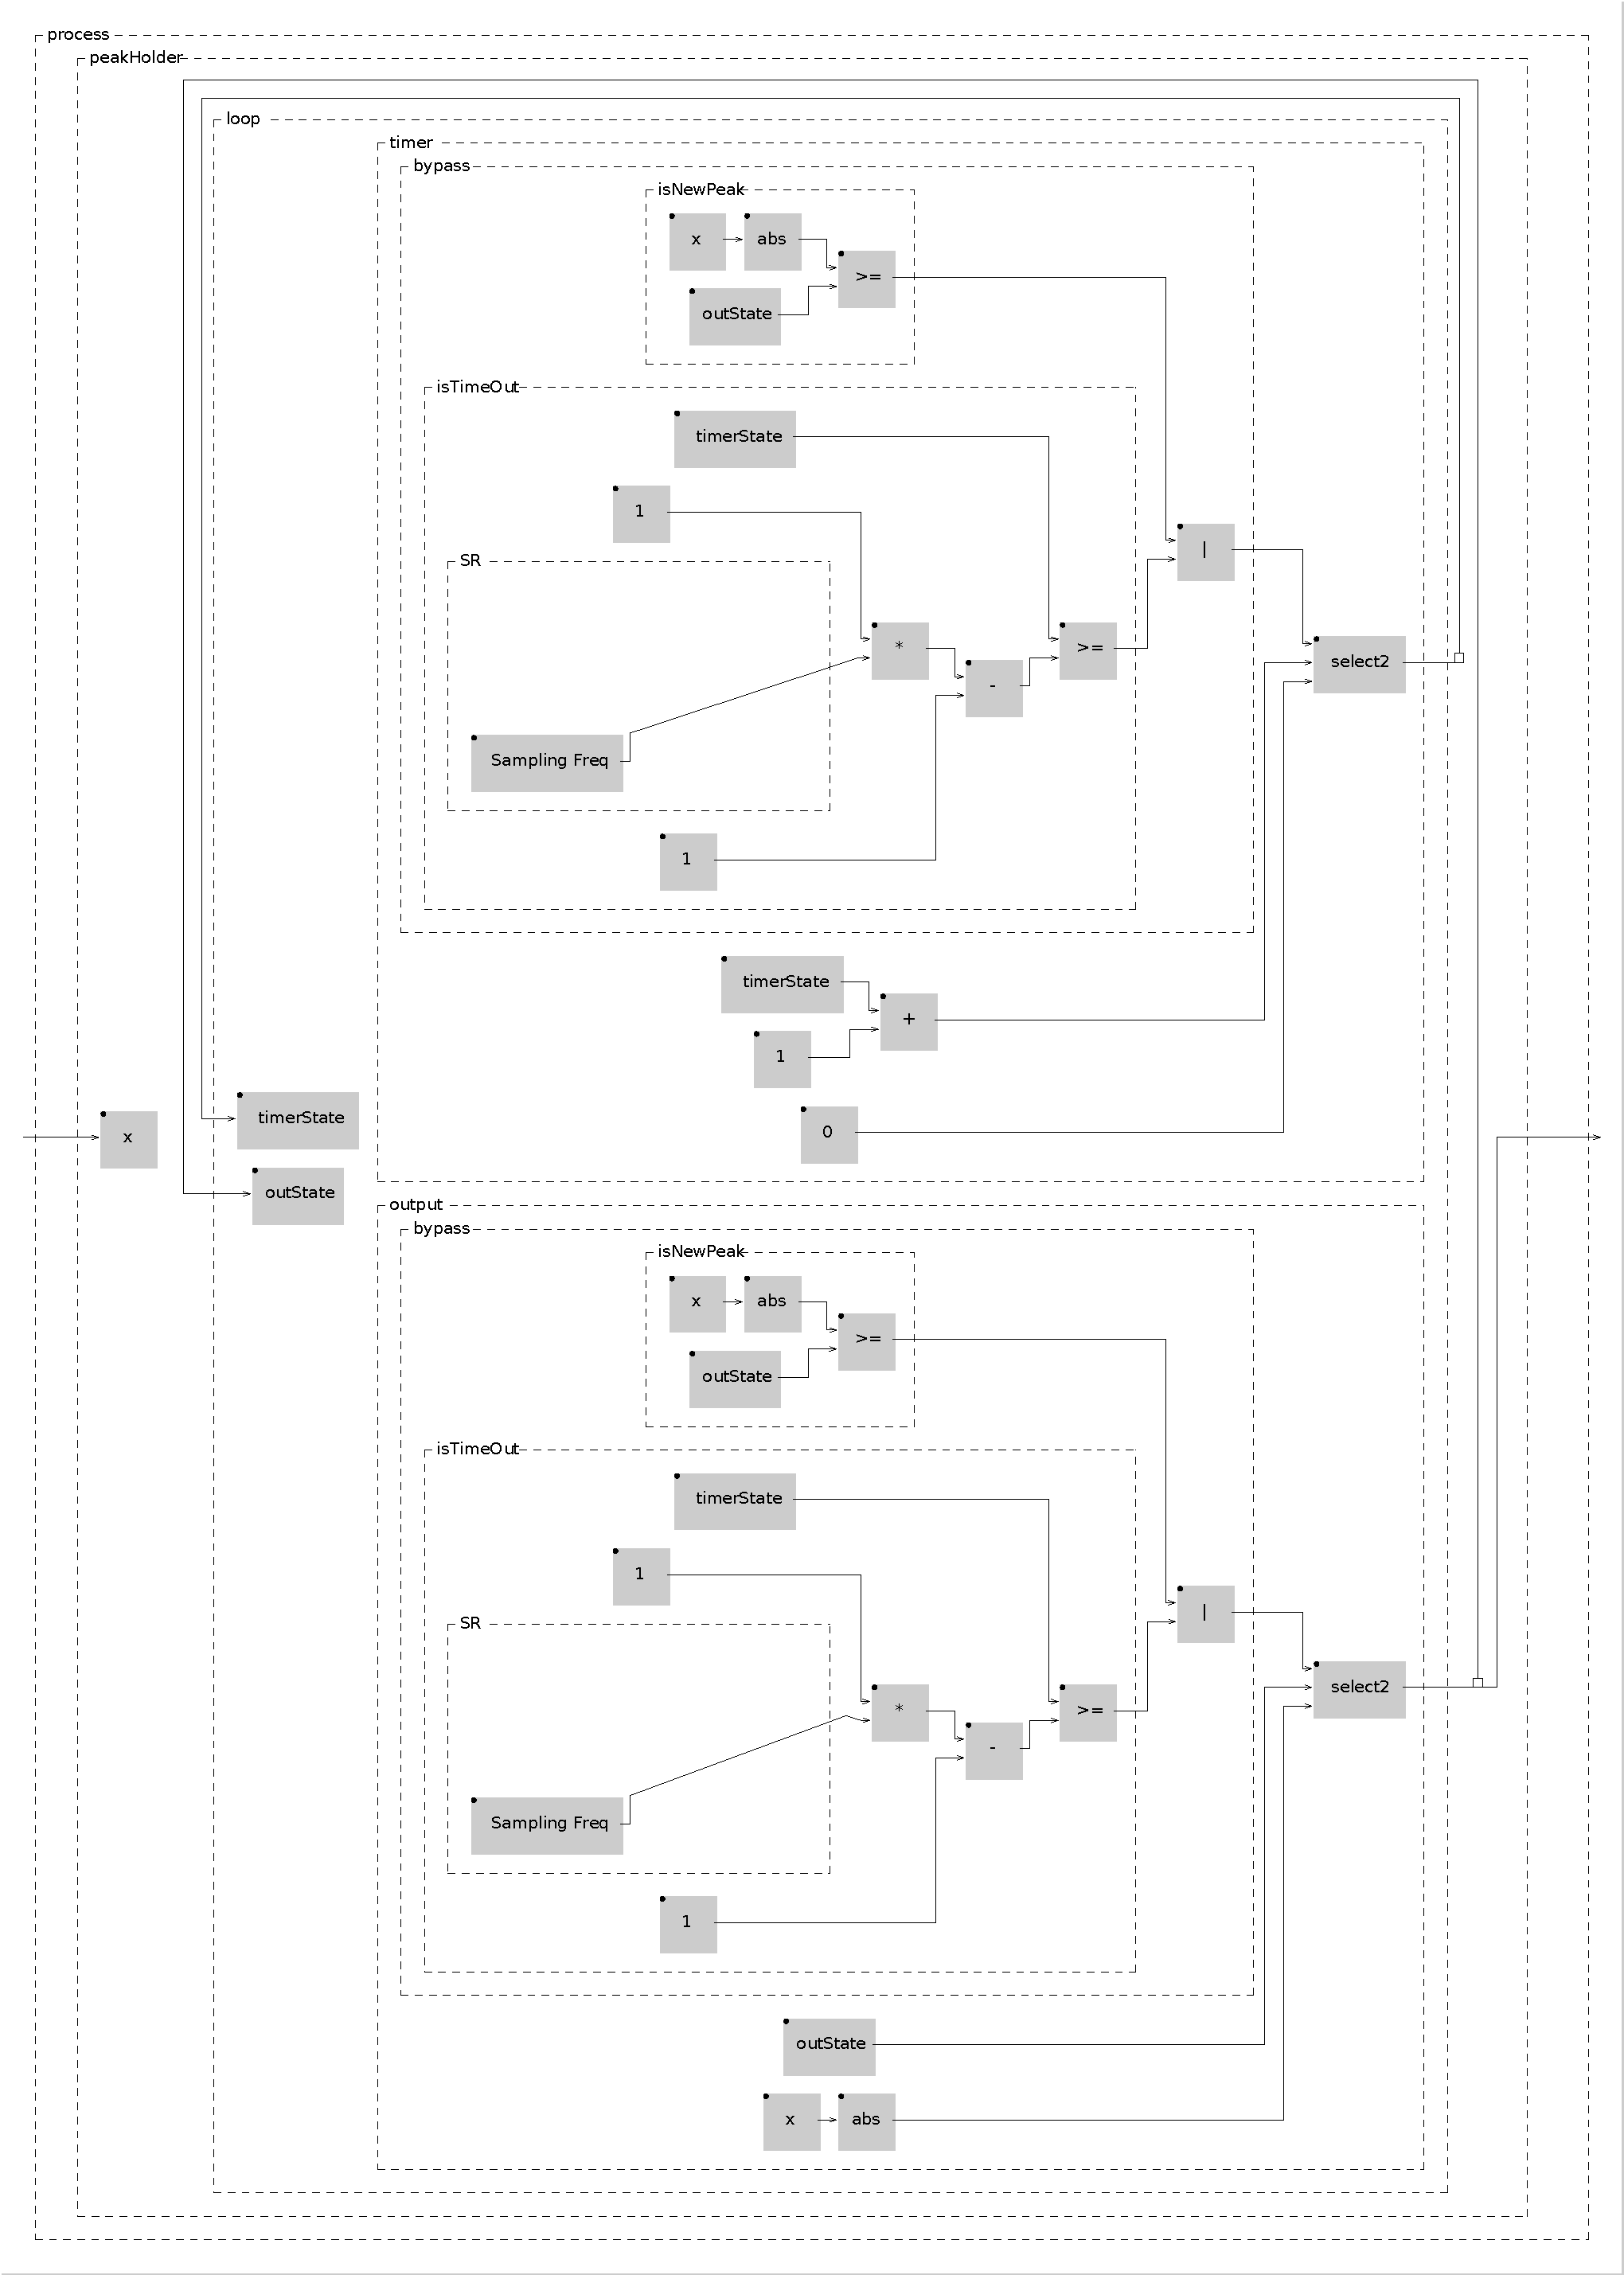
\includegraphics[width=15cm]{figures/PeakHolderAdaptive.pdf}
        \caption{Topologia del \textit{Peakholder} (adattivo) con Timer}
    \end{center}
    \vspace{0.5cm}
    \end{figure}

\clearpage 

Per concludere infine le unità sono combinate fra loro come a seguito,
formando nel loro insieme il \textit{Lookahead Limiter}.

\vspace{0.5cm} 
\lstinputlisting[breaklines, frame=trBL, caption={Algoritmo del \textit{Lookahead Limiter}}]
{codes/LookaheadLimiter.dsp}

Prima di concludere queste considerazioni a seguito qualche doverosa aggiunta.
Anche nell'Ecosistemico Udibile n.2, studio sul \emph{feedback}, di Agostino Di Scipio è presente 
una versione ottimizzata dell'algoritmo \textit{Peakholder}, che a differenza
del \textit{Peakholder} con il timer discusso precedentemente, viene chiamato come
\textit{Local Max}, e riporta l'ampiezza massima solamente al termine del \textit{time frame} che corrisponde
al reset del timer, senza necessità della complessa condizione vero/falso discussa precedentemente, 
ma a discapito di un tempo di ritardo dovuto all'analisi del valore massimo che viene riportato 
solo al termine del \textit{time frame}.
In partitura viene descritto come segue:

\begin{quote}
    \begin{itemize}
      \item local max = returns the maximum signal amplitude (absolute value) 
      in a given time frame; frame duration is dynamically adjusted: 
      the next frame duration is set at the end of the previous frame
    \end{itemize}
    \end{quote}

A seguito l'implementazione del \textit{Local Max} in Faust.

\vspace{0.5cm} 
\lstinputlisting[breaklines, frame=trBL, caption={Algoritmo del \textit{Local Max}}]
{codes/LocalMax.dsp}

\subsection{Conclusioni}
\label{sec:Conclusioni}

In conclusione, abbiamo avuto modo di approfondire alcuni dei principali meccanismi 
utilizzati da Dario Sanfilippo nel suo brano Order From Noise \textit{(Homage to Heinz Von Foerster)},
prendendo questo lavoro come caso di studio, con il fine di illustrare
alcune modalità e relazioni possibili per rendere un sistema autonomo e 
capace di manifestare comportamenti emergenti e complessità anche all'interno di uno 
spazio deterministico interamente costituito solo dal DSP nel software 
(che abbiamo chiamato qui col nome di spazio latente); 
inclusi metodi e strategie per la generazione delle relative non linearità,
e meccanismi adattivi per mantenere il sistema in una condizione di stabilità
controllata tramite algoritmi di \emph{feedback positivo} e \emph{negativo}.
Anche qui i meccanismi contenuti all'interno del brano ovviamente non si limitano solamente a questi,
ma si è cercato di approfondire le parti del sistema che riguardano l'\textit{Audio Information Processing};
così da fornire alcuni strumenti che rendano possibile affrontare il problema 
dell'adattattività e dell'\textit{adattattività dinamica}
all'interno dei CASes, lasciando comunque aperta la possibilità 
di poter approfondire il brano a partire
dai testi citati in bibliografia, che riportano anche le formule matematiche e la descrizione
per gli altri moduli e le altre unità del brano.